\chapter{SysML v1}
\section{Bevezetés}
Az OMG Systems Modeling Language (OMG SysML) egy általános felhasználású grafikus modellezési nyelv komplex rendszerek specifikálására, analízisére, tervezésére és verifikálására.
Ezen rendszerek taralmazhatnak hardver és szoftver elemeket, információt, személyeket, folyamatokat és létesítményeket.

A SysML eredetileg a SysML Partners' SysML Open Source Specification Project\footnote{https://sysml.org/sysml-partners/} által jött létre 2003-ban.
Később, 2006-ban az Object Management Group (OMG) adaptálta és adoptálta a SysML-t és az első verziót (SysML v1.0) 2007-ben jelent meg.

A SysML v1 az UML 2-es verziójának kiegészítése révén jött létre UML v2 profilként, amelyet a \ref*{fig:sysv1_uml}. ábra mutat be.

\begin{figure}
    \centering
    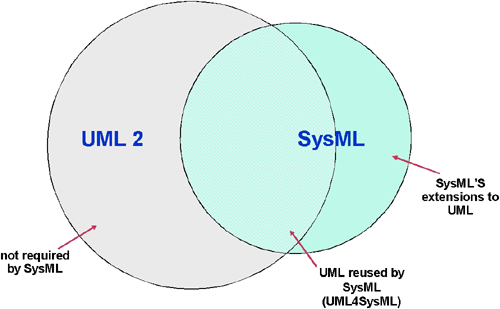
\includegraphics[width=80mm,keepaspectratio]{figures/SysmlV1_Figure-1-a.jpg}
    \caption{SysML v1 felépítése. Forrás: https://www.omgsysml.org/what-is-sysml.html}
    \label{fig:sysv1_uml}
\end{figure}

\section{A nyelv felépítése}
A nyelv diagramjai a \ref*{fig:sysv1_diag}. ábrán láthatók.

Egy blokk az alap építőelem a SysML-ben, ami reprezentálhat hardvert szoftvert, létesítményt, személyt vagy bármilyen rendszerelemet.

\begin{figure}
    \centering
    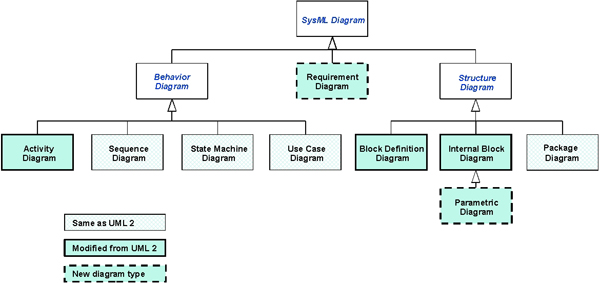
\includegraphics[width=150mm, keepaspectratio]{figures/SysmlV1_diag.jpg}
    \caption{SysML v1 diagrammok.}
    \label{fig:sysv1_diag}
\end{figure}